\documentclass{beamer}
\usepackage[italian]{babel}
\usepackage{pifont}
\usepackage{pgffor}
\usepackage{hyperref}
\usepackage{amssymb}
\usepackage{mathabx}

\usetheme{Madrid}
\usecolortheme{default}

\title[]{Implementation of a Python library that generalizes the CLUE algorithm}

\author[Simone Balducci]{Presented by: Simone Balducci \\ \vspace{3mm}}
\institute[]{Alma Mater Studiorum-Università di Bologna}
\date{November 1st 2022}

\begin{document}

\frame{\titlepage}

\begin{frame}
\frametitle{Goals of the project}
The goals of this project were to:
\begin{itemize}
	\item Generalize CLUE to N dimensions
	\item Bind the algorithm to Python
	\item Write a Python class ``clusterer" that executes CLUE
	\item Deploy the algorithm to a PyPi library
\end{itemize}
\end{frame}
\begin{frame}
\frametitle{Generalization to N dimensions}
To generalize the code, several steps were needed:
\begin{itemize}
	\item add the number of dimensions, Ndim, as a template parameter for all the classes
	\item introduce a new metric $\longrightarrow$ N-dimensional euclidian metric
	\item remove the parameters specific to the detector's geometry
	\item redefine the tiles
	\item rewrite the algorithms for the local density and the distance to higher 
	\item rewrite the mainRun functions
\end{itemize}
\end{frame}
\begin{frame}
\frametitle{Tiles}
\begin{itemize}
	\item originally, the tiles where calculated based on the detector's geometry
	\begin{itemize}
		\item[\ding{228}] now we want them to be calculated based on the points	
	\end{itemize}
	\item the number of tiles is calculated based on the desired average number of points per tile $\longrightarrow$ new constructor's input parameter
	\item the size of the tiles in each dimensions is calculated depending on the coordinate's range
	$$
		NTiles = 10, \ x_{min} = 1, \ x_{max} = 4 \ \longrightarrow \ \boxed{xbin_{size} = 0.3}
	$$
	\item the resulting tiles are all identical parallelepipeds
\end{itemize}
\end{frame}
\begin{frame}
\frametitle{Local density and distance to higher}
\begin{itemize}
	\item the original algorithm iterated through x and y bins
	\item we must find a way to iterate through a generic number of dimensions 
	\item we define a recursive function
		\begin{itemize}
			\item it calculates all the N dimensional bins in the given range
			\item executes the calculation (local density or NH) in each one
		\end{itemize}
\end{itemize}
\begin{center}
	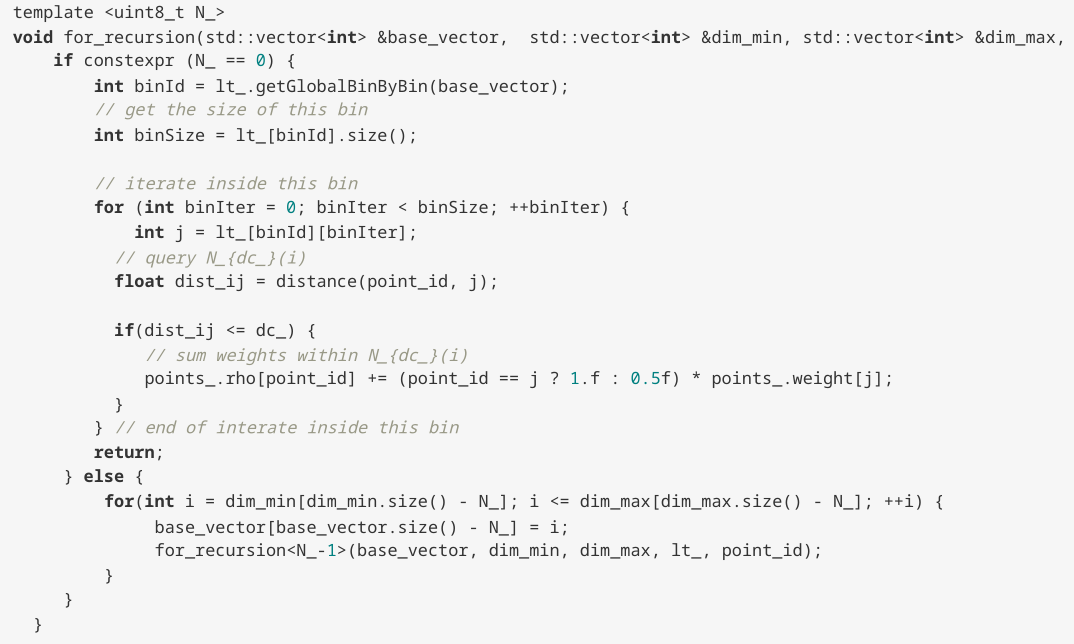
\includegraphics[scale=0.3]{recursion.png}
\end{center}	
\end{frame}
\begin{frame}
\frametitle{Local density and distance to higher}
\begin{itemize}
	\item we then use the recursive function to calculate the local density (or NH)
\end{itemize}
\begin{center}
	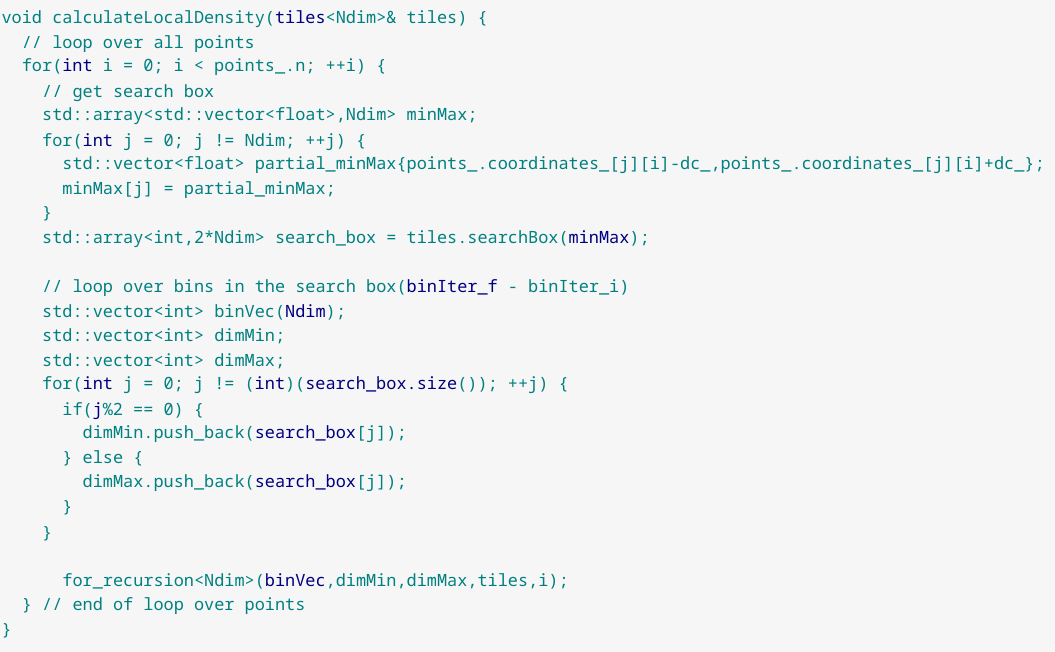
\includegraphics[scale=0.3]{localdensity.png}
\end{center}
\end{frame}
\begin{frame}
\frametitle{mainRun and run functions}
\begin{itemize}
	\item in C++ template parameters must be known at compile time
	\item in order to bind mainRun, the number of dimensions can't be a variable
	\item we define many ``run" functions, for which Ndim is known and constant
\end{itemize}
\begin{center}
	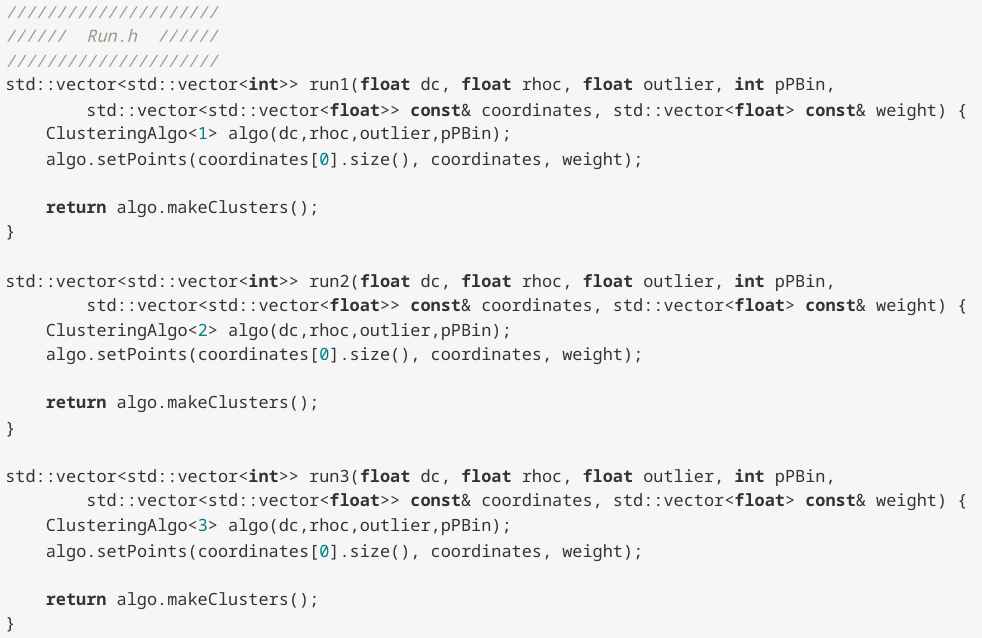
\includegraphics[scale=0.3]{run.png}
\end{center}
\end{frame}
\begin{frame}
\frametitle{mainRun and run functions}
\begin{itemize}
	\item mainRun takes Ndim as input parameter and uses it to call the right run function
\end{itemize}
\begin{center}
	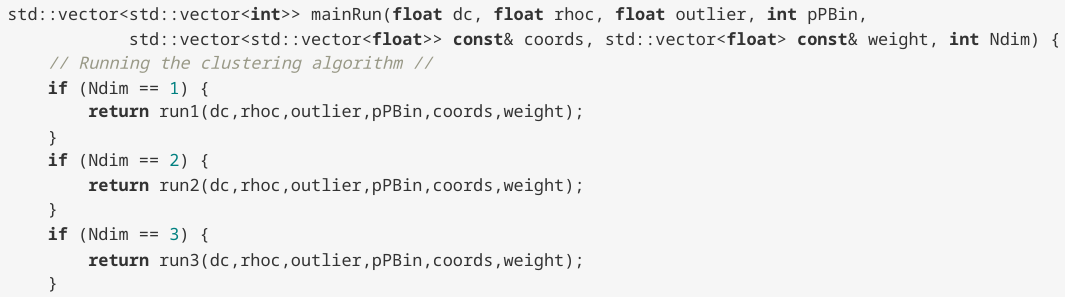
\includegraphics[scale=0.3]{mainRun.png}
\end{center}
\begin{itemize}
	\item the compiler is happy
\end{itemize}
\end{frame}
\begin{frame}
\frametitle{Binding}
\begin{itemize}
	\item the binding has been done with the use of Pybind11
	\item the binded function is mainRun
\end{itemize}
\begin{center}
	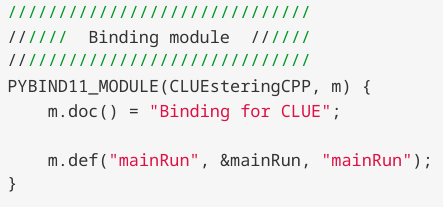
\includegraphics[scale=0.7]{binding.png}
\end{center}
\end{frame}
\begin{frame}
\frametitle{The \textit{clusterer} class}
In the library is defined a class named clusterer \\
The class contains some methods:
\begin{itemize}
	\item constructor	
	\item readData
	\item runCLUE
	\item inputPlotter 
	\item clusterPlotter 
	\item toCSV
\end{itemize}
\end{frame}
\begin{frame}
\frametitle{Execution times for different numbers of dimensions}
\begin{itemize}
	\item the execution times have a weird trend	
	\item nonetheless, the trend is upwards
\end{itemize}
\begin{center}
	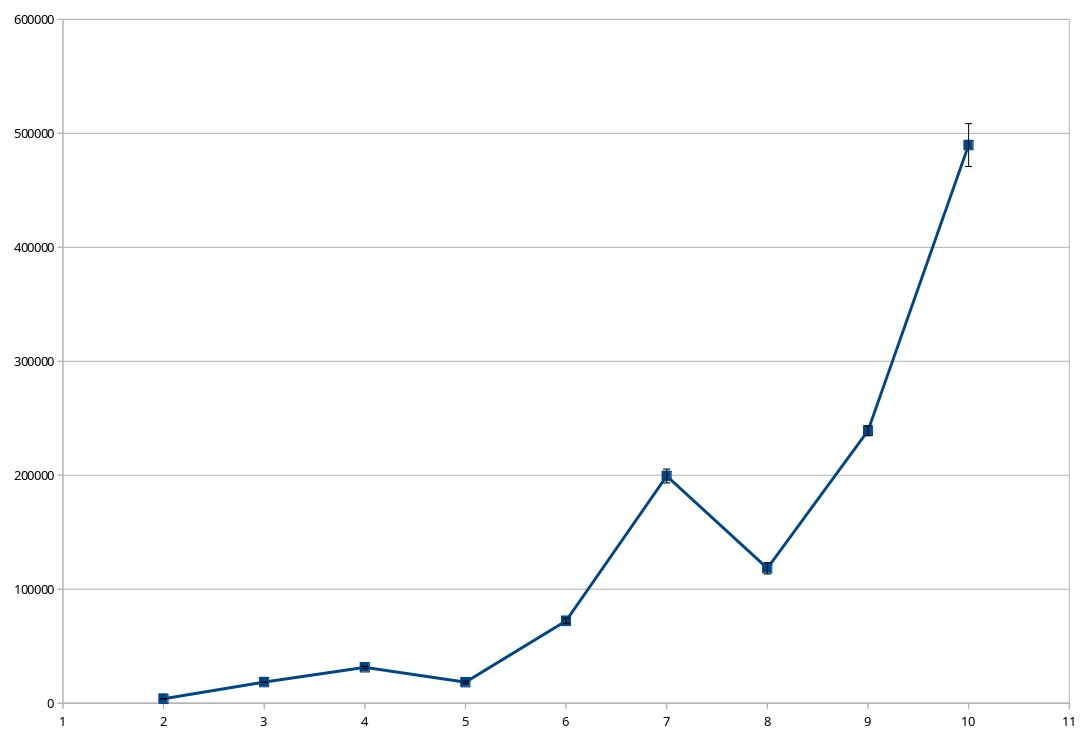
\includegraphics[scale=0.3]{Time_Scaling.jpg}
\end{center}
\end{frame}
\begin{frame}
\frametitle{Python library}
\begin{itemize}
	\item The library has been called CLUEstering
	\item It can already be found on PyPi
\end{itemize}
\begin{center}
	\url{https://pypi.org/project/CLUEstering/}
\end{center}
\end{frame}
\begin{frame}
\frametitle{Possible future developements}
\begin{itemize}
	\item better documentation and docstrings
	\item doing a preliminary calculation of the point density
		\begin{itemize}
			\item first estimation for the parameters
			\item tiles with variable size
		\end{itemize}
	\item optimization on the C++ side for better performance
	\item (maybe) run on GPU
\end{itemize}
\end{frame}

\end{document}
